\documentclass[10pt,a4paper]{article}
\usepackage[utf8]{inputenc}
\usepackage[T1]{fontenc}
\usepackage{amsmath}
\usepackage{amsfonts}
\usepackage{amssymb}
\usepackage{makeidx}
\usepackage{graphicx}
\usepackage{wrapfig}
\usepackage{mdframed}
\usepackage{xcolor}
\usepackage{tikz}
\usepackage{pgfplots}
\pgfplotsset{width=3in,compat=1.9}
\usepackage[left=1.00in, right=1.00in, top=1.00in, bottom=1.00in]{geometry}
\author{Tommaso Severini}
\title{Geometria analitica - Circonferenza}
\begin{document}
	\maketitle
	
		%% mdframed definizione
	\mdfdefinestyle{theoremstyle}{%
		linecolor=orange,linewidth=2pt,%
		frametitlerule=true,%
		frametitlebackgroundcolor=gray!20,
		innertopmargin=\topskip,
	}
	\mdtheorem[style=theoremstyle]{definition}{Definition}
	
	In geometria una circonferenza è il luogo geometrico di punti del piano equidistanti da un punto fisso detto centro.
	
	\begin{center}
		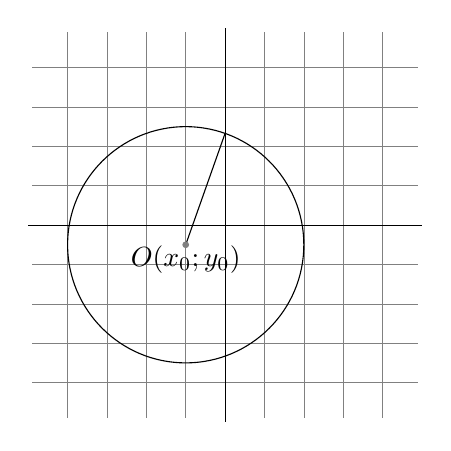
\begin{tikzpicture}
			\draw[step=0.5cm,gray,very thin] (-2.45,-2.45) grid (2.45,2.45);
			\draw (-2.5,0) -- (2.5,0);
			\draw (0,-2.5) -- (0,2.5);
			\draw (-0.5,-0.25) circle [radius=1.5cm];
			\draw (-0.5,-0.25) -- (0, 1.1642135623731);
			
			\filldraw [gray] (-0.5,-0.25) circle [radius=1pt];
			\draw (-0.5,-0.5) node [text height=4pt] {$O(x_0 ; y_0)$};
		\end{tikzpicture}

	\end{center}
	
	In un sistema di riferimento cartesiano, la circonferenza di centro $O(x_0;y;0)$ e raggio $r$ è caratterizzata dall'equazione:
	\begin{definition}[Equazione di una circonferenza]
	\centering	$(x-x_0) + (y-y_0) = r^2 $
	\end{definition}
	
	Espandendo i quadrati di binomi e ordinando i termini in ordine di esponente decrescente, otteniamo la forma canonica dell'equazione scritta sopra:
	
	\begin{definition}[Forma canonica]
		\centering	$x^2 + y^2 + ax + by + c = 0$
		
		Dalle sostituzioni effettuate ne conviene che:
		\begin{itemize}
			\item $-2x_0 = a$ ovvero $ x_0 = -\frac{a}{2}$
			\item $-2y_0 = b$ ovvero $ y_0 = -\frac{b}{2}$
			\item $c = x_0^2 + y_0^2 -r^2$ ovvero $ r = \sqrt{x_0^2 + y_0^2 -c}$
		\end{itemize}
	\end{definition}
	
\end{document}